\documentclass[a4paper,11pt]{article}
\usepackage{amsmath,amsthm,amsfonts,amssymb,amscd,amstext,vmargin,graphics,graphicx,tabularx,multicol} 
\usepackage[francais]{babel}
\usepackage[utf8]{inputenc}  
\usepackage[T1]{fontenc} 
\usepackage{pstricks-add,tikz,tkz-tab,variations}
\usepackage[autolanguage,np]{numprint} 
\usepackage{calc}
\usepackage{mathrsfs}

\usepackage{cancel}

\setmarginsrb{1.5cm}{0.5cm}{1cm}{0.5cm}{0cm}{0cm}{0cm}{0cm} %Gauche, haut, droite, haut
\newcounter{numexo}
\newcommand{\exo}[1]{\stepcounter{numexo}\noindent{\bf Exercice~\thenumexo} : }
\reversemarginpar

\newcommand{\bmul}[1]{\begin{multicols}{#1}}
\newcommand{\emul}{\end{multicols}}

\newcounter{enumtabi}
\newcounter{enumtaba}
\newcommand{\q}{\stepcounter{enumtabi} \theenumtabi.  }
\newcommand{\qa}{\stepcounter{enumtaba} (\alph{enumtaba}) }
\newcommand{\initq}{\setcounter{enumtabi}{0}}
\newcommand{\initqa}{\setcounter{enumtaba}{0}}

\newcommand{\be}{\begin{enumerate}}
\newcommand{\ee}{\end{enumerate}}
\newcommand{\bi}{\begin{itemize}}
\newcommand{\ei}{\end{itemize}}
\newcommand{\bp}{\begin{pspicture*}}
\newcommand{\ep}{\end{pspicture*}}
\newcommand{\bt}{\begin{tabular}}
\newcommand{\et}{\end{tabular}}
\renewcommand{\tabularxcolumn}[1]{>{\centering}m{#1}} %(colonne m{} centrée, au lieu de p par défault) 
\newcommand{\tnl}{\tabularnewline}

\newcommand{\trait}{\noindent \rule{\linewidth}{0.2mm}}
\newcommand{\hs}[1]{\hspace{#1}}
\newcommand{\vs}[1]{\vspace{#1}}

\newcommand{\N}{\mathbb{N}}
\newcommand{\Z}{\mathbb{Z}}
\newcommand{\R}{\mathbb{R}}
\newcommand{\C}{\mathbb{C}}
\newcommand{\Dcal}{\mathcal{D}}
\newcommand{\Ccal}{\mathcal{C}}
\newcommand{\mc}{\mathcal}

\newcommand{\vect}[1]{\overrightarrow{#1}}
\newcommand{\ds}{\displaystyle}
\newcommand{\eq}{\quad \Leftrightarrow \quad}
\newcommand{\vecti}{\vec{\imath}}
\newcommand{\vectj}{\vec{\jmath}}
\newcommand{\Oij}{(O;\vec{\imath}, \vec{\jmath})}
\newcommand{\OIJ}{(O;I,J)}


\newcommand{\reponse}[1][1]{%
\multido{}{#1}{\makebox[\linewidth]{\rule[0pt]{0pt}{20pt}\dotfill}
}}

\newcommand{\titre}[5] 
% #1: titre #2: haut gauche #3: bas gauche #4: haut droite #5: bas droite
{
\noindent #2 \hfill #4 \\
#3 \hfill #5

\vspace{-1.6cm}

\begin{center}\rule{6cm}{0.5mm}\end{center}
\vspace{0.2cm}
\begin{center}{\large{\textbf{#1}}}\end{center}
\begin{center}\rule{6cm}{0.5mm}\end{center}
}



\begin{document}
\pagestyle{empty}
\titre{Séance d'exercices: Résolution d'équation du premier degré}{}{}{3ème}{}

\vspace*{0.2cm}



\exo\\

Noah veut acheter des livres qui coûtent le même prix.\\
S'il en achète 7, il lui manque 1,20 euros. S'il en achète 6, il lui reste 3,50 euros.\\

Quel est le prix d'un livre ?\\


\color{red}
On appelle $x$ le prix d'un livre.\\

L'équation est la suivante : \hspace*{1cm} $7x-1,20= 6x+3,50$ 


$$7x-1,20-6x= 6x+3,50-6x$$

$$x-1,20= 3,50$$

$$x-1,20+1,20=3,50+1,20$$

$$x=4,70$$

Un livre coûte 4,70 euros.\\

 \color{black}
\vspace*{0.5cm}

\exo \\

Deux frères, Marc et Jean, possèdent chacun un jardin. L'aire du jardin de Marc vaut les $\dfrac{3}{4}$ de l'aire du jardin de Jean. Les deux frères possèdent en tout 1 470 $ m^{2} $.\\

Quelles sont les aires des jardins de Marc et de Jean  ?\\

\color{red}


On appelle $x$, l'aire du terrain de Jean.\\

Pour trouver l'équation, il faut choisir une grandeur qui peut être exprimée de deux façons différentes.\\

Ici, il s'agit de l'aire du jardin qu'ils ont à eux 2.\hspace*{1cm} \textbf{Il y a 1 470 $m^{2}$ en tout}.\\

Mais cela peut aussi s'écrire : \textbf{Aire de Jean + Aire de Marc.}\\

On sait que :
\bi
\item \textcolor{green}{Aire de Jean = x}

\item l'aire du jardin de Marc vaut les $\dfrac{3}{4}$ de l'aire du jardin de Jean. , à savoir \textcolor{blue}{Aire de Marc = $\dfrac{3}{4}x$ }

\ei

L'équation est donc la suivante : \hspace*{1cm} $ \textcolor{green}{Aire de Jean } + \textcolor{blue}{Aire de Marc}  = 1 470$\\

$$ x + \dfrac{3}{4}x = 1470$$


$$ \dfrac{4}{4}x + \dfrac{3}{4}x = 1470$$

$$ \dfrac{7}{4}x = 1470$$

$$ \dfrac{\dfrac{7}{4}x}{\dfrac{7}{4}} = \dfrac{1470}{\dfrac{7}{4}}$$


$$x = \dfrac{1470}{\dfrac{7}{4}}$$


$$x =1470 \times \dfrac{4}{7}$$

$$x =840$$

Donc, l'aire du terrain de Jean vaut 840 $m^{2}$.\\

Pour Marc : $\dfrac{3}{4} \times 840 = 630 m^{2}$ \hspace*{1.5cm}\textbf{Vérification :} 840 + 630 = 1 470.\\



\color{black}


  \exo \\ x désigne un nombre supérieur à 1.\\
ABCD est un trapèze dont les côtés parallèles [AD] et [BC] ont des longueurs variables.\\

Existe-t-il un nombre x pour lequel ABCD est un
parallélogramme ? \textit{Si oui, préciser la nature de ABCD.}\\

\begin{center}
\includegraphics[scale=0.8]{exoequation.eps} 

\end{center}
 
 
 


\color{red}

Pour savoir si ABCD peut être un parallélogramme, il faut trouver une valeur de $x$ pour que $5x-3=x+5$\\

On résout l'équation :\\

$$ 5x-3-x=5 $$

$$ 4x-3=5 $$


$$ 4x=5 +3$$


$$ 4x=8$$


$$ x=\dfrac{8}{4}$$


$$ x=2$$

Si $x=2$ alors ABCD est un parallélogramme\\

On a alors : $5x-3 = 5 \times 2 - 3 = 7$ et $x+5 = +5 =7$\\

ABCD est un parallélogramme qui possède 2 côtés consécutifs de même longueur, c'est donc un losange.\\



\end{document}
